\documentclass[11pt]{article}

\usepackage[review]{acl}

\usepackage{times}
\usepackage{latexsym}
\usepackage[T1]{fontenc}
\usepackage[utf8]{inputenc}
\usepackage{microtype}
\usepackage{inconsolata}
\usepackage{graphicx}
\usepackage{booktabs}
\usepackage{multirow}
\usepackage{caption}
\usepackage{amsmath}
\usepackage{amssymb}
\usepackage{float}

\hyphenation{com-ple-men-tary correct-ness sig-nal}

% Stubs so the file compiles in both review (lineno active) and final (no lineno) modes.
\providecommand{\linenumbers}{}
\providecommand{\nolinenumbers}{}

% Fix lineno bleeding into floats (only meaningful in review mode)
\makeatletter
\let\old@table\table
\let\old@endtable\endtable
\renewenvironment{table}[1][]{%
  \nolinenumbers\old@table[#1]%
}{%
  \old@endtable\linenumbers%
}
\makeatother

\title{Tracing Functional Correctness in DLMs with Sparse Autoencoders}

\author{Guan-Ming Chiu \\
  National Taiwan University \\
  \texttt{gmchiu@arbor.ee.ntu.edu.tw} \\\And
  Jeng-Yue Liu \\
  Carnegie Mellon University \\
  \texttt{buffettl@andrew.cmu.edu} \\}

\begin{document}
\maketitle
\raggedbottom

\begin{abstract}
Prior probing of diffusion language models (DLMs) suggests that correctness signal grows monotonically through denoising.
Using DLM-Scope sparse autoencoders, we instead trace the signal feature by feature across two DLMs and four tasks.
Sparse fail-vs-pass concentration appears in task-dependent phases: code and structural tasks form a broad mid-denoising plateau, while reasoning tasks emerge only at the final state.
On LLaDA-8B / MBPP, a dense step sweep across seeds confirms the plateau spans steps $48$--$116$ with multiple sub-steps reaching $p{<}0.05$ and a within-plateau hand-off from one persistent feature to another at the late phase.
The peak phase agrees across LLaDA-8B and Dream-7B on $3/4$ tasks, although most individual cross-grid cells do not reach per-step significance.
However, single- and multi-feature steering fails to flip correctness in a small pilot intervention set, suggesting these sparse features are diagnostic under our current protocol rather than directly controllable knobs.
\end{abstract}

\section{Introduction}

Diffusion language models (DLMs) generate text by iteratively denoising a fully masked sequence over $\sim$100 steps \citep{austin2021d3pm,sahoo2024simple,lou2024discrete,nie2025llada,ye2025dream}.
\citet{chiu2026probe} shows that simple classifiers trained on hidden states gain $0.08$--$0.11$ AUC predicting functional correctness as denoising proceeds, framing the process as a monotonic sharpening of an aggregate scalar.
This view leaves a basic question unanswered: \emph{which} representational components carry the failure signal, and \emph{when} during denoising do they form?

\paragraph{Contributions.}
\begin{itemize}
\setlength{\itemsep}{0pt}
\item \textbf{Mid-denoising plateau.}
LLaDA-8B / MBPP has a broad plateau over steps $48$--$116$ (3-seed dense sweep), with \texttt{f15601} top-ranked at the early plateau and \texttt{f3892} at the late plateau.
\item \textbf{Phase agreement.}
Peak phase agrees across LLaDA-8B and Dream-7B on $3/4$ tasks, while per-cell significance is concentrated in the strongest LLaDA-MBPP condition.
\item \textbf{Steering null.}
Single-, top-5, and reverse feature interventions fail to flip correctness in a pilot intervention sweep.
\end{itemize}
Code and figures will be released on acceptance.

\section{Related Work}

Discrete diffusion and masked DLMs generate by iteratively denoising masked tokens rather than left-to-right continuation \citep{austin2021d3pm,sahoo2024simple,lou2024discrete,nie2025llada,ye2025dream}, and prior probing work on the same models and tasks studies aggregate hidden-state predictability and reports monotonic gains in correctness AUC through denoising.
SAEs decompose residual streams into sparse named features and have been used primarily to interpret autoregressive LMs \citep{bricken2023monosemanticity,cunningham2024sae,gao2024scaling}; DLM-Scope extends this toolkit to DLMs with Top-$K$ SAEs \citep{makhzani2014topk,gao2024scaling} trained on masked-position residuals across mask rates $t\!\sim\!U(0,1)$ (\emph{Mask-SAE}), so the full denoising trajectory is in distribution \citep{dlmscope2026}.
Recent AR SAE studies report both successful steering for refusal and instruction following \citep{obrien2024refusal,he2025saif} and cautions that contrastive features may track lexical correlates or that steering degrades unrelated capabilities \citep{galichin2025reasoning,korznikov2025roguescalpel}.
We reuse the DLM-Scope SAEs to ask whether the scalar correctness trend on DLMs decomposes into temporally localised sparse features, treating the steering question as open rather than presumed causal.

\section{Method}
\label{sec:method}

\paragraph{Models and SAEs.}
LLaDA-8B \citep{nie2025llada} (block-wise unmasking, block length 32) and Dream-7B \citep{ye2025dream} (global linear schedule) both denoise a $\!\le\!256$-token generation region over $T{=}128$ steps conditioned on a fully visible prompt.
We use the DLM-Scope L26 LLaDA-mask SAE and L23 Dream-mask SAE (trainer index 2, $d_{\mathrm{sae}}{=}16{,}384$, $K{=}160$).
The AR comparison (DLM-Scope L23 SAE on Qwen-2.5-7B \citep{qwen2.5}) is a single-token reference point, not a trajectory: we encode the last-prompt-token residual once per sample as a single-step analog of the DLM's pre-generation state.

\paragraph{Data.}
We reuse cached hidden states and functional-correctness labels from \citet{chiu2026probe}: MBPP-sanitized (257) \citep{austin2021program}, JSON schema (272), GSM8K (1{,}319) \citep{cobbe2021gsm8k}, and ARC-Challenge (1{,}172) \citep{clark2018arc}, generated with seed $0$ and $T{=}128$ steps.
Hidden states are mean-pooled over four equal-length generation regions at seven checkpoint steps $\{0,1,4,16,32,64,127\}$.

\paragraph{Per-step SAE encoding.}
At each (model, step, layer) cell we take the region-mean hidden state $h \in \mathbb{R}^{d}$ per sample and encode it:
$z = \mathrm{TopK}\!\bigl(\mathrm{ReLU}\!\left(W_{\mathrm{enc}}(h{-}b_{\mathrm{dec}}) + b_{\mathrm{enc}}\right)\!\bigr) \in \mathbb{R}^{d_{\mathrm{sae}}}$,
with $W_{\mathrm{enc}}\!\in\!\mathbb{R}^{d_{\mathrm{sae}}\times d}$, $W_{\mathrm{dec}}\!\in\!\mathbb{R}^{d\times d_{\mathrm{sae}}}$, $b_{\mathrm{enc}}\!\in\!\mathbb{R}^{d_{\mathrm{sae}}}$, $b_{\mathrm{dec}}\!\in\!\mathbb{R}^{d}$,
and $\mathrm{TopK}$ keeps the $K{=}160$ largest entries.
Feature $i$ is \emph{active} on a sample iff $z_i\!>\!0$.

\paragraph{Fail-vs-pass enrichment.}
Let $\mathcal{F},\mathcal{P}$ be the fail and pass sets at a cell.
Feature $i$'s enrichment is the difference of active rates,
$\mathrm{enr}(i) = \tfrac{1}{|\mathcal{F}|}\!\sum_{s \in \mathcal{F}} \mathbb{1}[z^{(s)}_i\!>\!0] - \tfrac{1}{|\mathcal{P}|}\!\sum_{s \in \mathcal{P}} \mathbb{1}[z^{(s)}_i\!>\!0]$.
We use the top-20 most fail-enriched features as the analysis subset per cell.

\paragraph{Cluster discriminability with permutation null.}
We run KMeans on the fail samples for $K\!\in\!\{2,3,4,5\}$ using the top-20 features (continuous activations) and report the silhouette of the best $K$.
The permutation null shuffles labels $1000\times$, \emph{re-selects} the top-20 features on each shuffled label set, then recomputes silhouette, controlling for the post-hoc feature selection.
We report $p = \Pr[\mathrm{silhouette}_{\mathrm{perm}}\!\ge\!\mathrm{silhouette}_{\mathrm{obs}}]$.
The silhouette is computed on fails only and measures sub-structure within failures, not fail-vs-pass separability directly.
We therefore interpret it as \emph{concentration of failure modes} in a selected sparse subspace, and cross-check fail/pass separability with supervised AUC in the same subspace (Appendix~\ref{sec:appendix_auc_compare}, per-fold selection).

\paragraph{Steering.}
We write \emph{fail$\to$pass} for a sample whose label flips from fail to pass after intervention, and \emph{pass$\to$fail} for the reverse pass-side regression.
Given a target feature $i^\star$ and strength $\alpha$, a forward hook on the SAE layer's transformer block re-encodes the residual at every step $t \!\ge\! t_0$, reads $z_{i^\star}$, and in-place subtracts $\alpha \cdot z_{i^\star}\!\cdot\! W_{\mathrm{dec}}[:, i^\star]$.
$\alpha\!<\!0$ amplifies the feature (reverse intervention); for multi-feature steering we sum contributions over a set of indices.
A zero-out smoke test (force $h\!\leftarrow\!0$) confirms the hook propagates: it garbles trailing tokens but leaves the early-committed function body intact, consistent with LLaDA committing blocks 0--3 by step $\sim\!48$.

\section{Results}
\label{sec:trajectory}

\begin{figure}[t]
  \centering
  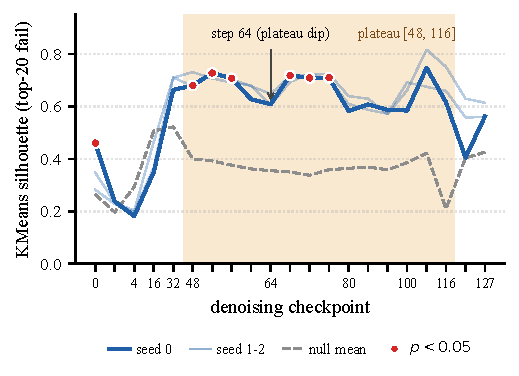
\includegraphics[width=0.95\columnwidth]{../figures/fig1_trajectory.pdf}
  \caption{LLaDA-8B / MBPP: KMeans silhouette on the top-20 fail-enriched features vs.\ permutation null mean across denoising steps. All $21$ checkpoints (anchors $\{0,1,4,16,32\}$, plateau $\{48$--$80\}$, post-plateau $\{84$--$124\}$, final $127$) are from a single new-prompt generation run; faint lines overlay two additional generation seeds (Appendix~\ref{sec:appendix_seed}). Shaded region marks the mid-denoising plateau $[48, 116]$ where most steps reach $p{<}0.05$; step 64 sits inside the plateau as a local dip, not a sharp peak.}
  \label{fig:trajectory}
\end{figure}

\begin{figure*}[t]
  \centering
  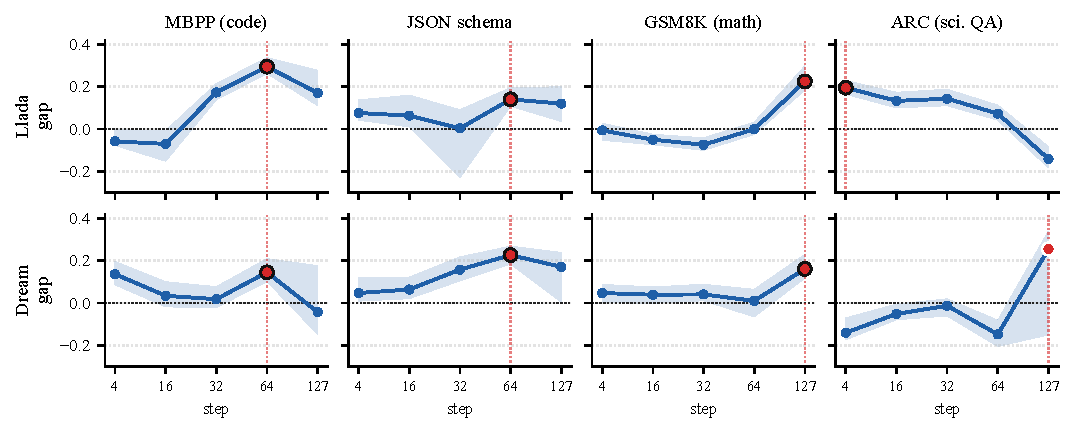
\includegraphics[width=\textwidth]{../figures/fig2_cross.pdf}
  \caption{Cross-model $\times$ cross-task trajectory grid. Each panel plots signal-to-null gap (observed KMeans silhouette minus permutation null mean) across denoising steps for one (model, task) cell;
  red marker = peak gap step; black outline = $p{<}0.05$ permutation significance.
  Code (MBPP) and structural (JSON) tasks peak at mid-denoising (step 64) on both DLMs.
  Math (GSM8K) and---on Dream---science QA (ARC) peak at late denoising (step 127).
  The peak step shows task-level agreement across LLaDA-8B and Dream-7B on three of four tasks; only ARC disagrees (LLaDA peak step 4, Dream step 127).}
  \label{fig:cross}
\end{figure*}

\paragraph{Mid-denoising plateau.}
Figure~\ref{fig:trajectory} reports a $21$-step trajectory for LLaDA-MBPP from a single generation run, with three seeds (Appendix~\ref{sec:appendix_seed}): anchors $\{0,1,4,16,32\}$, plateau dense $\{48,52,\ldots,80\}$, post-plateau dense $\{84,92,\ldots,124\}$, and final state $127$.
Rather than a sharp peak at step 64, the trajectory shows a broad plateau spanning steps $48$--$116$: the signal-to-null gap stays in $[+0.19, +0.41]$ throughout this range and only collapses at step $124$ as the model approaches its final state.
\texttt{f15601} is the top-1 fail-enriched feature at $7/9$ of the early-plateau dense steps and remains dominant through step $100$; in the late-plateau steps $108$--$116$ it is replaced by \texttt{f3892} as the top marker, indicating a within-plateau hand-off rather than feature swapping outside the plateau.
At steps $0$--$16$ the top fail feature changes every step (Appendix~\ref{sec:appendix_persist}), consistent with the residual stream not yet encoding committed-token decisions when most positions are still masked.
\citet{chiu2026probe} reports that aggregate raw-probe AUC \emph{monotonically} increases over these same steps (for LLaDA / MBPP, from $\sim$$0.75$ at step 0 to $\sim$$0.84$ at step 64); the feature-level plateau is thus invisible to scalar probing.

\paragraph{Cross-model $\times$ cross-task phase agreement.}
\label{sec:cross}
Figure~\ref{fig:cross} reports the full $2{\times}4$ trajectory grid (full numeric table in Appendix~\ref{sec:appendix_grid_full}).
Three archetypes emerge across cells.
\textbf{Mid-denoising peak} (signal peaks at step 64): LLaDA-MBPP ($+0.31$), LLaDA-JSON ($+0.14$), Dream-JSON ($+0.23$), Dream-MBPP ($+0.15$).
This is the shape of the persistent-feature trajectory described in \S\ref{sec:trajectory}: a fail-discriminative cluster crystallises during the middle of denoising and partially dissipates by step 127.
\textbf{Late-denoising peak} (signal peaks at step 127): LLaDA-GSM8K ($+0.22$), Dream-GSM8K ($+0.16$), Dream-ARC ($+0.26$).
Here the cluster signal is weak or below null at mid-denoising and only emerges near the final state, consistent with reasoning tasks requiring more denoising before the failure signature crystallises.
\textbf{Early-decline} (LLaDA-ARC peaks at step 4, $+0.20$): an outlier where the cluster appears only at the earliest steps and decays thereafter.
The peak position shows \emph{task-level agreement across DLMs}: three of four tasks (MBPP, JSON, GSM8K) have matching peak step across LLaDA and Dream; only ARC differs across models.
At the feature level this mirrors the structural-vs-reasoning emergence split of \citet{chiu2026probe}---structural and code tasks form features mid-denoising; reasoning tasks form them late---now visible as a peak position rather than a continuous AUC curve.
Appendix~\ref{sec:appendix_grid} summarises the 12 (DLM and AR) cells at step 64;
across the full grid only two cells reach $p{<}0.05$ at any single step (LLaDA-MBPP step 64, Qwen-JSON step 64).
Thus the cross-DLM result should be read as a descriptive phase-alignment claim, with statistical support strongest for the LLaDA-MBPP plateau.

\paragraph{Top-feature drift and persistence.}
On LLaDA-8B / MBPP, pairwise Jaccard of the top-20 sets is high among steps 0--4 ($\ge 0.48$, before committed-token information is available), moderate between 32 and 64 ($0.29$, the plateau regime), and falls to $0.14$ between 64 and 127.
On the sparse 7-step grid, only \texttt{f15601} appears at all three peak-or-later steps; the dense sweep (Appendix~\ref{sec:appendix_dense}) sharpens this by showing \texttt{f15601} is the top-1 fail-enriched feature at 7 of 9 dense steps in $[48,80]$, supporting a persistent statistical marker rather than feature swapping inside the plateau.
Outside the plateau, the sparse support reorganises as denoising commits different token blocks: early features are unstable, the compact failure marker \texttt{f15601} crystallises during 48--76, and the final state at step 127 spreads signal over a different set of atoms.
The temporal peak is therefore a concentration effect in sparse feature space, not merely a monotonic increase in correctness information.
Full Jaccard matrix and per-feature enrichment trajectories are in Figure~\ref{fig:drift_app} (Appendix~\ref{sec:appendix_persist}).

\begin{table}[!t]
  \centering\small
  \setlength{\tabcolsep}{4pt}
  \begin{tabular}{llcc}
    \toprule
    condition & from & fail$\to$pass & pass$\to$fail \\
    \midrule
    baseline & none & 0/8 & 0/3 \\
    suppress \texttt{f15601} & s64 & 0/8 & 0/3 \\
    suppress \texttt{f15601} & s16 & 0/8 & 0/3 \\
    suppress top-5 & s64 & 0/8 & 0/3 \\
    reverse \texttt{f15601} & s64 & 0/8 & 0/3 \\
    \bottomrule
  \end{tabular}
  \caption{Pilot steering intervention summary on LLaDA-8B / MBPP; entries show flips / evaluated cases.
  Conditions: baseline (no intervention); suppress \texttt{f15601} at step 64 (peak) or step 16 (pre-peak); suppress the top-5 fail features at step 64; reverse intervention ($\alpha\!=\!-5$) amplifying \texttt{f15601} at step 64.
  No condition converts any fail$\to$pass or pass$\to$fail.}
  \label{tab:steering}
\end{table}

\paragraph{Pilot steering null result.}
\label{sec:steer}
We test whether the cluster-level feature signature can be directly controlled, restricting to LLaDA-8B / MBPP where the cluster reaches significance.
We run five intervention conditions on cluster-1 fail cases and pass-side regression controls (Table~\ref{tab:steering}; entries report flips / evaluated cases).
Suppressing the persistent peak feature \texttt{f15601} ($\alpha{=}5$) at the peak window (step 64) or before formation onset (step 16) yields \emph{zero} fail$\to$pass conversions and \emph{zero} pass$\to$fail regressions.
Multi-feature suppression of the top-5 fail features at step 64 is also null.
Reverse intervention ($\alpha{=}-5$, amplifying \texttt{f15601}) is null on pass-side cases as well.
The hook does propagate---a separate zero-out test ($h{\leftarrow}0$ at $t\!\ge\!0$) destroys trailing generation while leaving the function body intact, consistent with LLaDA committing blocks 0--3 by step $\sim\!48$.
This pilot result does not rule out causal roles for these features, but it does show that correctness is not flipped by ablating one direction or a small set of directions under this intervention protocol.

\section{Discussion}

\paragraph{Statistical vs.\ causal features.}
\texttt{f15601} fires on $65\%$ of LLaDA-8B / MBPP fails vs.\ $27\%$ of passes at step 64---a $\sim\!6.6\sigma$ per-feature effect---yet ablating it (or the top-5 fail features) in any of four intervention windows flips no label.
The cluster signature is useful as a diagnostic, but our intervention evidence is insufficient to treat this sparse direction as a knob that controls functional correctness.
This contrasts with positive AR steering results on refusal and instruction following \citep{obrien2024refusal,he2025saif} but is consistent with reports that activation steering may degrade unrelated capabilities \citep{korznikov2025roguescalpel}.
More decisive causal tests would need paired counterfactual replacements, multi-layer interventions, or attribution from output-level correctness back to the SAE layer.

\paragraph{Why do peak times differ by task?}
By step 64, LLaDA has unmasked blocks 0--3 (the function signature and early body) but not blocks 4--7.
For code and structural tasks, this mid-state appears to be where fail-vs-pass information is maximally factored into a small set of sparse features: enough tokens are settled to expose the failure mode, while later tokens still carry uncertainty.
By step 127 the signal still exists but is less concentrated in the top-20 sparse features.
For GSM8K and Dream-ARC, by contrast, the sparse cluster peaks only at the final checkpoint, suggesting that reasoning failures become feature-separable later than format or code failures.
This task-dependent timing also explains why a single intervention window is unlikely to control correctness across tasks.

\section{Conclusion}

Tracing functional-correctness signal feature by feature reveals temporal structure that scalar probes miss: sparse failure markers form task-dependent phases.
Code and structural tasks form a mid-denoising plateau, while reasoning tasks peak at the final state; this peak-phase pattern agrees across LLaDA-8B and Dream-7B on three of four tasks, with strongest support on LLaDA-MBPP.
In that cell, a 3-seed dense sweep confirms a steps $48$--$116$ plateau and a late hand-off from \texttt{f15601} to \texttt{f3892}.
Pilot linear-feature interventions do not flip correctness, so these sparse features are currently diagnostic markers; causal control likely requires stronger interventions.

\section*{Limitations}

\paragraph{SAE coverage.}
All findings depend on a single DLM-Scope Mask-SAE per model (L26 for LLaDA, L23 for Dream), trained with mask rate $t\!\sim\!U(0,1)$ on masked-position residuals.
The full denoising trajectory is therefore in distribution, but features extracted at other layers, the Unmask-SAE trained on already-revealed positions, or higher-capacity dictionaries ($K{>}160$) may surface different failure correlates.
Early-step instability (steps 0--16) reflects the residual stream not yet encoding committed-token decisions rather than SAE distribution shift.

\paragraph{Feature semantics.}
We identify persistent dictionary atoms such as \texttt{f15601} and \texttt{f3892} by statistical enrichment and temporal persistence, not by human-validated semantic labels.
The present experiments therefore support a claim about when sparse failure markers concentrate, but they do not name the underlying error modes captured by each feature.
Manual cluster inspection or activation-maximising examples would be needed to turn these feature IDs into interpretable failure categories.

\paragraph{Permutation test interpretation.}
Our permutation null re-selects the top-20 fail features on each shuffled label set before recomputing silhouette.
This is conservative (any post-hoc selection procedure that could find clusters on random labels is included in the null), and it inflates the null mean noticeably (e.g.\ $0.36$ for LLaDA-8B / MBPP at step 64).
A consequence is that only two of twelve cells reach $p<0.05$ at an individual step on the sparse 7-grid even though the DLM grid shows systematic plateau structure.
The dense sweep in Appendix~\ref{sec:appendix_dense} shows 7 of 9 sub-steps in $[48, 76]$ reach $p<0.05$ on LLaDA-MBPP, so sparse-grid per-step significance is an underestimate; we present our cross-model claims as plateau-shape claims rather than per-cell significance.

\paragraph{Steering coverage.}
Our intervention sweep tests four denoising windows, two feature-set sizes (single and top-5), and one magnitude pair ($\alpha\!\in\!\{+5,-5\}$) at a single SAE layer per DLM (L26 for LLaDA, L23 for Dream).
We do not test multi-layer joint interventions, non-linear projections, or feature-selection strategies that use the per-step top-1 (where the top fail feature differs from \texttt{f15601}).
Effect-size diagnostics (Appendix~\ref{sec:appendix_effect}) confirm the intervention reaches $\|\Delta h\| / \|h\| \in [4.4\%, 14.8\%]$ at the SAE-layer residual, so the null result is not because the perturbation was silent; rather, a negative result on this protocol is narrower than a negative result on all possible linear-feature interventions.

\paragraph{Cluster $K$ and choice of metric.}
We use silhouette on KMeans with $K\!\in\!\{2,3,4,5\}$ and report the best $K$ per cell.
On LLaDA-8B / MBPP the best $K$ is $2$ at every step; on Dream / MBPP step 64 the best $K$ is $3$ with one small (size-26) sub-cluster.
Appendix~\ref{sec:appendix_sensitivity} reports top-$N$ and clustering-method sensitivity: silhouette and significance are robust across $N\!\in\!\{10,20,30,50\}$ at step $68$ (the plateau peak) and across KMeans/Agglomerative/HDBSCAN.
A labels-hidden $K{=}2$ test on the full fail+pass set yields ARI $\approx 0$, confirming the silhouette measures within-fail sub-structure rather than fail/pass separability; supervised AUC in Appendix~\ref{sec:appendix_auc_compare} reports the latter.

\paragraph{Cross-model comparison.}
LLaDA uses block-wise unmasking with block length 32, whereas Dream uses a global linear schedule.
At a matched checkpoint step, the spatial distribution of unmasked tokens differs between the models, so step-axis comparisons in Figure~\ref{fig:cross} reflect approximate denoising-progress alignments rather than identical model states.
We do not attempt to map between block-wise commit fractions and global mask fractions on a per-sample basis.
Our AR baseline (Qwen-2.5-7B) uses last-prompt-token hidden states; this is the natural single-token analog of the DLM's pre-generation state but is not a temporal trajectory.

\paragraph{Task coverage.}
Functional correctness is verified across four tasks (MBPP, JSON schema, GSM8K, ARC), but this still covers only a small slice of DLM use cases.
Generalising the task-dependent peak finding to other open-ended tasks (instruction following, dialog, multi-turn reasoning) requires task-appropriate functional metrics and additional DLMs.

\paragraph{Sample size and seed dependence.}
Cluster sample sizes are limited by the number of fail cases per (model, dataset) cell: MBPP has $\sim$$140$ fails per DLM, but GSM8K has fewer than $250$ each.
A three-seed sensitivity check on LLaDA-MBPP (Appendix~\ref{sec:appendix_seed}) shows pass/fail counts vary by at most $\pm 3$ samples and the plateau structure is preserved across seeds; the temporal-oscillation phenomenon noted in concurrent DLM work \citep{wang2025time} would primarily affect borderline samples, which our seed-stability check is consistent with.

\paragraph{Causal interpretation.}
Even with the negative steering result, our conclusion that ``\texttt{f15601} is a diagnostic correlate rather than a directly controllable cause under our protocol'' is interpretation-dependent.
A more decisive test would be a counterfactual experiment that surgically replaces the feature direction with a paired pass-cluster feature direction at the peak step, or a gradient-based attribution that traces logit differences back to the SAE layer.
We leave such causal-mechanistic follow-up to future work.

\bibliography{custom}

\appendix

\section{Top-Feature Persistence Across Steps}
\label{sec:appendix_persist}
Figure~\ref{fig:drift_app} shows the pairwise Jaccard of top-20 fail features between denoising steps and the enrichment trajectory of three illustrative features for LLaDA-8B / MBPP.
Table~\ref{tab:persist} reports the per-step silhouette, permutation $p$, and top fail-enriched feature.
\texttt{f15601} is the only feature among the top-20 at all three peak-or-later steps (32, 64, 127).
\begin{figure*}[t]
  \centering
  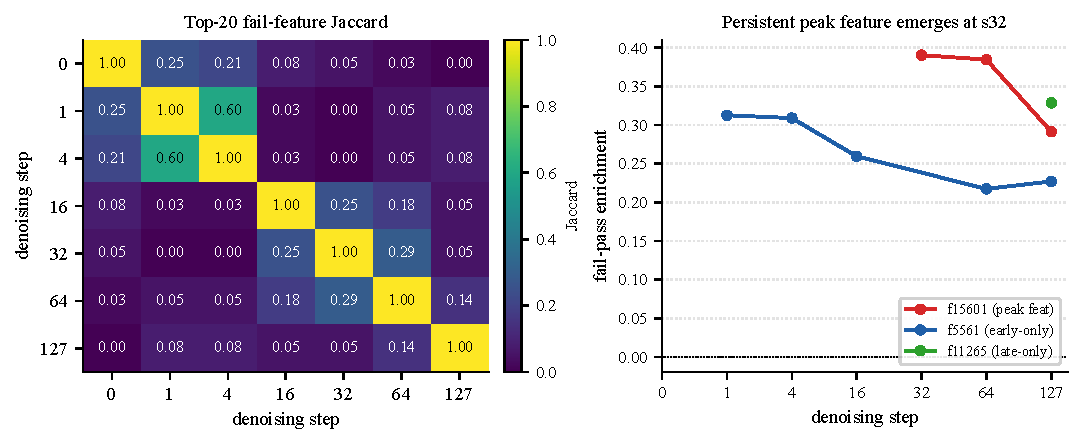
\includegraphics[width=0.92\textwidth]{../figures/fig4_feature_drift.pdf}
  \caption{Left: pairwise Jaccard of top-20 fail features between denoising steps. Right: enrichment trajectory of \texttt{f15601} (persistent peak), \texttt{f5561} (early only), and \texttt{f11265} (final only).}
  \label{fig:drift_app}
\end{figure*}
\begin{table}[H]
  \centering\small
  \begin{tabular}{rrll}
    \toprule
    step & best $K$ & silhouette / $p$ & top fail feat \\
    \midrule
    0 & 2 & 0.271 / 0.418 & f6421 ($+0.295$) \\
    1 & 2 & 0.220 / 0.793 & f5561 ($+0.313$) \\
    4 & 2 & 0.231 / 0.727 & f5561 ($+0.309$) \\
    16 & 2 & 0.440 / 0.541 & f3892 ($+0.326$) \\
    32 & 2 & 0.702 / 0.118 & f15601 ($+0.391$) \\
    64 & 2 & 0.662 / \textbf{0.033} & f15601 ($+0.385$) \\
    127 & 2 & 0.601 / 0.144 & f11265 ($+0.329$) \\
    \bottomrule
  \end{tabular}
  \caption{LLaDA-8B / MBPP per-step diagnose summary.}
  \label{tab:persist}
\end{table}

\section{Qualitative Cluster Inspection}
\label{sec:appendix_cluster_examples}

Table~\ref{tab:cluster_examples} shows illustrative LLaDA-MBPP failures from the two step-64 fail clusters.
We re-generated the first ten fail samples from each cluster with the baseline LLaDA decoding setup and re-ran the MBPP tests.
Cluster 0 yields 3 assertion failures, 2 syntax errors, 4 name errors, and 1 value error; cluster 1 yields 5 assertion failures, 4 name errors, and 1 type error.
The examples are not intended as human-validated feature labels; they only show that both sparse clusters contain concrete functional failures, ranging from malformed code to plausible but semantically wrong implementations.

\begin{table*}[t]
  \centering\small
  \setlength{\tabcolsep}{4pt}
  \resizebox{\textwidth}{!}{%
  \begin{tabular}{cllp{0.38\textwidth}}
    \toprule
    cluster & characteristic features & task & observed failure \\
    \midrule
    0 & \texttt{f11404}, \texttt{f9798}, \texttt{f189}, \texttt{f496}, \texttt{f8825}
      & closest smaller number
      & Generates a long case split that returns $n$ for small inputs instead of $n{-}1$, failing assertions. \\
    0 & \texttt{f11404}, \texttt{f9798}, \texttt{f189}, \texttt{f496}, \texttt{f8825}
      & unique element in sorted array
      & Produces malformed pointer-update code with a syntax error. \\
    1 & \texttt{f189}, \texttt{f492}, \texttt{f3320}, \texttt{f11404}, \texttt{f15601}
      & remove first/last occurrence
      & Removes only boundary characters and misses interior first/last occurrences, failing assertions. \\
    1 & \texttt{f189}, \texttt{f492}, \texttt{f3320}, \texttt{f11404}, \texttt{f15601}
      & lowercase underscore regex
      & Uses \texttt{re.compile} without importing \texttt{re}, causing a \texttt{NameError}. \\
    \bottomrule
  \end{tabular}
  }
  \caption{Illustrative generated failures from LLaDA-MBPP step-64 fail clusters. Error-type counts are computed over 10 regenerated failures per cluster; full generated outputs and errors are saved in \texttt{mbpp\_llada/cluster\_failure\_examples.json} on the Modal \texttt{probe-results} volume.}
  \label{tab:cluster_examples}
\end{table*}

\section{Step-64 Cross-grid Snapshot}
\label{sec:appendix_grid}
Table~\ref{tab:grid} summarises silhouette + permutation $p$ across the 4 datasets $\times$ 3 models grid at step 64, complementing the trajectory-shape claim in Appendix~\ref{sec:appendix_grid_full}.
\begin{table}[H]
  \centering\small
  \setlength{\tabcolsep}{3.2pt}
  \begin{tabular}{lccc}
    \toprule
    dataset & LLaDA & Dream & Qwen \\
    \midrule
    mbpp & 0.66 / \textbf{0.033} & 0.50 / 0.128 & 0.16 / 0.106 \\
    json & 0.58 / 0.195 & 0.77 / 0.135 & 0.22 / \textbf{0.007} \\
    gsm8k & 0.38 / 0.432 & 0.29 / 0.449 & 0.15 / 0.315 \\
    arc & 0.43 / 0.312 & 0.18 / 0.882 & 0.13 / 0.343 \\
    \bottomrule
  \end{tabular}
  \caption{Silhouette / permutation $p$ at step 64 per condition; bold $p<0.05$. Full trajectory in Table~\ref{tab:grid_full}.}
  \label{tab:grid}
\end{table}

\section{Generation and Probing Details}
\label{sec:appendix_generation}

\paragraph{Denoising procedure.}
Both models run 128 denoising steps.
LLaDA uses block-based unmasking: the generation region is divided into blocks of 32 tokens, and each block is denoised sequentially over $128 / (\text{gen\_length} / 32)$ steps per block.
Within each block, the model selects the most confident tokens to unmask at each step.
Dream uses a global linear schedule: at step $i$, the fraction of tokens to unmask is determined by a linearly decreasing timestep schedule from $t=1$ to $t=\epsilon$, and the most confident masked tokens are unmasked globally.

\paragraph{Prompt construction.}
For JSON schema, we prepend a system prompt containing the target schema and append a JSON code-fence marker as a generation prefix.
For GSM8K, the system prompt instructs the model to solve step-by-step and end with \texttt{\#\#\#\#} followed by the numeric answer.
Both models use their respective chat templates.
A complete prompt example for each task is shown in Figure~\ref{fig:prompt_examples}.

\begin{figure}[!b]
\small
\begin{tabular}{p{0.93\columnwidth}}
\toprule
\textit{JSON schema (LLaDA chat template)} \\[2pt]
\texttt{[BOS] system\textbackslash n You are a helpful assistant that answers in JSON. Here's the JSON schema you must adhere to:\textbackslash n <schema>\textbackslash n \{schema\} \textbackslash n </schema>\textbackslash n user\textbackslash n \{user input\}\textbackslash n assistant\textbackslash n ```json\textbackslash n} \\[2pt]
\midrule
\textit{GSM8K (Dream chat template)} \\[2pt]
\texttt{[BOS] im\_start system\textbackslash n Solve the math problem step by step. End your answer with \#\#\#\# followed by the final numeric answer. im\_end\textbackslash n im\_start user\textbackslash n \{question\} im\_end\textbackslash n im\_start assistant\textbackslash n} \\
\bottomrule
\end{tabular}
\caption{Schematic prompt examples after each model's chat template is applied (special tokens shown as plain words for readability; the actual tokens used are model-specific control tokens). The generation region (128--512 masked tokens) is appended after the final assistant marker. Both models share the same system/user content; only the wrapping tokens differ.}
\label{fig:prompt_examples}
\end{figure}

\paragraph{Hidden state extraction.}
At each of the 7 checkpoint steps $\{0, 1, 4, 16, 32, 64, 127\}$, we run a forward pass with \mbox{\texttt{output\_hidden\_states=True}} and extract the residual stream at the SAE layer.
The generation region is partitioned into 4 equal-length position regions and mean-pooled within each region, producing a $d$-dimensional vector per region (4096 for LLaDA, 3584 for Dream and Qwen).
The region-mean is passed through the DLM-Scope SAE for feature analysis (\S\ref{sec:method}).

\paragraph{Steering hook implementation.}
The steering hook is registered on the SAE-layer transformer block via \texttt{register\_forward\_hook}.
The hook receives the tuple output, re-encodes \texttt{output[0]} through the SAE in-place, computes $\alpha \cdot z_{i^\star} \cdot W_{\mathrm{dec}}[:, i^\star]$ and subtracts the contribution.
A counter and per-step diagnostic prints confirm the hook fires $T{=}128$ times per generation (once per denoising step) and that the modification magnitude $\|\Delta h\|$ is non-zero.

\paragraph{Computational resources.}
All generation, encoding, and steering experiments use NVIDIA A100 (80GB) GPUs on Modal.
Models are loaded in bfloat16; SAE weights cast to bfloat16 for the steering hook.
Total compute: approximately 40 A100-hours across all reported experiments.

\paragraph{Reproducibility and determinism.}
Generation uses seed $0$; both LLaDA and Dream commit the highest-confidence masked positions deterministically, so the fail/pass partition per cell is reproducible across runs.
Hidden states are cached as bfloat16 tensors; SAE encoding reads from the dense residual cache on demand, so top-20 selection, KMeans, and permutation null are rerunnable without re-invoking either DLM.
The permutation null uses $1000$ shuffles per cell with a fixed permutation seed offset, so silhouette $p$-values are themselves reproducible.

\section{Full Cross-grid Trajectory}
\label{sec:appendix_grid_full}

Table~\ref{tab:grid_full} reports the signal-to-null gap (KMeans silhouette $-$ permutation null mean) at each of the five denoising checkpoints, for both DLMs $\times$ four tasks.
The peak step per cell is bolded; the only DLM peak with $p{<}0.05$ is LLaDA-8B / MBPP at step 64.
The table separates the trajectory-shape claim from per-step significance: modest gaps can still support the timing pattern when the same task peaks at the same denoising phase across both DLMs.

\begin{table*}[t]
  \centering\small
  \setlength{\tabcolsep}{5pt}
  \begin{tabular}{ll|rrrrr|l}
    \toprule
    model & task & $s{=}4$ & $s{=}16$ & $s{=}32$ & $s{=}64$ & $s{=}127$ & peak \\
    \midrule
    \multicolumn{8}{l}{\textit{LLaDA-8B}} \\
    & mbpp & $-0.06$ & $-0.07$ & $+0.18$ & $\mathbf{+0.31}$ & $+0.18$ & s64 \\
    & jsonschema & $+0.08$ & $+0.06$ & $+0.01$ & $\mathbf{+0.14}$ & $+0.12$ & s64 \\
    & gsm8k & $-0.01$ & $-0.05$ & $-0.08$ & $-0.00$ & $\mathbf{+0.22}$ & s127 \\
    & arc & $\mathbf{+0.20}$ & $+0.13$ & $+0.14$ & $+0.08$ & $-0.14$ & s4 \\
    \midrule
    \multicolumn{8}{l}{\textit{Dream-7B}} \\
    & mbpp & $+0.15$ & $+0.03$ & $+0.02$ & $\mathbf{+0.15}$ & $-0.03$ & s64 \\
    & jsonschema & $+0.04$ & $+0.06$ & $+0.16$ & $\mathbf{+0.23}$ & $+0.17$ & s64 \\
    & gsm8k & $+0.05$ & $+0.04$ & $+0.04$ & $+0.01$ & $\mathbf{+0.16}$ & s127 \\
    & arc & $-0.14$ & $-0.05$ & $-0.02$ & $-0.15$ & $\mathbf{+0.26}$ & s127 \\
    \bottomrule
  \end{tabular}
  \caption{Signal-to-null gap (observed silhouette $-$ permutation null mean) at five denoising checkpoints across the $2{\times}4$ (DLM, task) grid.
  Bold marks the peak step per cell.
  Cross-DLM peak-step agreement: MBPP (both s64), JSON (both s64), GSM8K (both s127); only ARC disagrees (LLaDA s4 vs Dream s127).}
  \label{tab:grid_full}
\end{table*}

\section{Per-condition Trajectory Detail}
\label{sec:appendix_cross_tables}

Table~\ref{tab:cross_traj} reports per-step silhouette, permutation $p$-value, and top fail feature for the four (DLM, task) conditions not detailed in Appendix~\ref{sec:appendix_persist}.
Two patterns are worth flagging.
Dream-7B / JSON schema concentrates on \texttt{f6326}, which is the top-1 fail-enriched feature at four of five checkpoint steps; this mirrors the persistent-feature behaviour seen for \texttt{f15601} on LLaDA-MBPP and supports the cross-DLM peak-step claim at the feature level.
In LLaDA-8B / GSM8K and LLaDA-8B / ARC after step 32 no single feature surfaces as a stable top-1 marker (dashes in the table); the cluster signal there is spread across multiple weakly-enriched features rather than concentrated on one atom, consistent with the negative single-feature steering result in \S\ref{sec:steer}.

\begin{table}[H]
  \centering\small
  \setlength{\tabcolsep}{4pt}
  \begin{tabular}{rrll}
    \toprule
    step & $K$ & silhouette / $p$ & top fail feat \\
    \midrule
    \multicolumn{4}{l}{\textit{Dream-7B / MBPP} (peak s64; below null at s127)} \\
    4 & 2 & 0.420 / 0.107 & f15414 ($+0.272$) \\
    16 & 2 & 0.413 / 0.231 & f6326 ($+0.342$) \\
    32 & 2 & 0.451 / 0.407 & f10891 ($+0.408$) \\
    64 & 3 & 0.497 / 0.128 & f6326 ($+0.421$) \\
    127 & 2 & 0.333 / 0.460 & f15414 ($+0.270$) \\
    \midrule
    \multicolumn{4}{l}{\textit{Dream-7B / JSON schema} (peak s64, $+0.23$ gap)} \\
    4 & 2 & 0.344 / 0.256 & f6326 ($+0.427$) \\
    16 & 2 & 0.401 / 0.213 & f10823 ($+0.433$) \\
    32 & 2 & 0.572 / 0.121 & f6326 ($+0.419$) \\
    64 & 2 & 0.773 / 0.135 & f6326 ($+0.420$) \\
    127 & 3 & 0.475 / 0.109 & f233 ($+0.349$) \\
    \midrule
    \multicolumn{4}{l}{\textit{LLaDA-8B / GSM8K} (late peak; s127 spike $+0.22$ gap)} \\
    4 & 3 & 0.190 / 0.394 & f2519 ($+0.197$) \\
    16 & 3 & 0.175 / 0.629 & f13085 ($+0.192$) \\
    32 & 2 & 0.255 / 0.661 & --- ($-$) \\
    64 & 2 & 0.379 / 0.432 & --- ($-$) \\
    127 & 2 & 0.701 / 0.197 & --- ($+0.224$ gap) \\
    \midrule
    \multicolumn{4}{l}{\textit{LLaDA-8B / ARC} (anomalous s4 peak, $+0.20$ gap)} \\
    4 & 2 & 0.627 / 0.079 & f4643 ($+0.186$) \\
    16 & 2 & 0.532 / 0.227 & f3892 ($+0.243$) \\
    32 & 2 & 0.480 / 0.155 & --- ($+0.142$ gap) \\
    64 & 2 & 0.427 / 0.312 & --- ($+0.075$ gap) \\
    127 & 2 & 0.316 / 0.784 & --- ($-0.142$ gap) \\
    \bottomrule
  \end{tabular}
  \caption{Per-step diagnose for the four (DLM, task) conditions complementing Table~\ref{tab:persist}. Dashes mark no single feature surfaces as the top-1 marker (cluster persists across multiple weakly-enriched features).}
  \label{tab:cross_traj}
\end{table}

\section{Single-feature vs.\ Raw-probe AUC}
\label{sec:appendix_auc_compare}

We compare the cross-validated AUC of (i) the single most-fail-enriched SAE feature, (ii) top-$N$ SAE features (logistic regression with per-fold selection), and (iii) a raw-probe baseline (PCA-64 + LR on the same hidden state) across all 12 cells (Table~\ref{tab:auc_compare}).
Raw-probe AUC dominates in 11 of 12 cells; the only SAE wins (Qwen / MBPP, Dream / ARC) are cells where the raw probe is itself near chance.
Top-20 SAE features recover roughly $85$--$95\%$ of the raw-probe AUC, suggesting sparse atoms carry most but not all of the signal in the dense residual.
This complements the negative steering finding (\S\ref{sec:steer}): even at optimal feature selection, sparse linear features under-represent the information that determines correctness.

\begin{table}[!b]
  \centering\scriptsize
  \setlength{\tabcolsep}{3pt}
  \begin{tabular}{llcccc}
    \toprule
    model & dataset & top-1 & top-5 & top-20 & raw \\
    \midrule
    \multicolumn{6}{l}{\textit{LLaDA-8B}} \\
    & mbpp & 0.59 & 0.73 & 0.73 & \textbf{0.82} \\
    & jsonschema & 0.67 & 0.66 & 0.69 & \textbf{0.81} \\
    & gsm8k & 0.69 & 0.71 & 0.72 & \textbf{0.77} \\
    & arc & 0.61 & 0.65 & 0.66 & \textbf{0.71} \\
    \midrule
    \multicolumn{6}{l}{\textit{Dream-7B}} \\
    & mbpp & 0.70 & 0.69 & 0.73 & \textbf{0.82} \\
    & jsonschema & 0.68 & 0.74 & 0.78 & \textbf{0.80} \\
    & gsm8k & 0.57 & 0.61 & 0.66 & \textbf{0.70} \\
    & arc & 0.49 & 0.54 & 0.56 & \textbf{0.57} \\
    \midrule
    \multicolumn{6}{l}{\textit{Qwen-2.5-7B (AR baseline)}} \\
    & mbpp & 0.57 & \textbf{0.66} & 0.59 & 0.61 \\
    & jsonschema & 0.59 & 0.66 & 0.71 & \textbf{0.75} \\
    & gsm8k & 0.59 & 0.66 & 0.71 & \textbf{0.75} \\
    & arc & 0.56 & 0.59 & 0.65 & \textbf{0.74} \\
    \bottomrule
  \end{tabular}
  \caption{Per-cell 5-fold cross-validated AUC at step 64 predicting functional correctness from top-$N$ SAE features (logistic regression, per-fold top-$N$ selection fitted on training folds only) vs.\ raw-probe baseline (PCA-64 fitted on training folds only + LR, applied to the \emph{same} SAE-layer hidden state). Bold marks the per-cell maximum.}
  \label{tab:auc_compare}
\end{table}

\section{Dense Temporal Sweep on MBPP}
\label{sec:appendix_dense}

We re-generate MBPP on both DLMs and capture hidden states at $9$ dense checkpoints in $[48, 80]$ (every $4$ steps) and an additional $6$ checkpoints in $[84, 124]$ (every $8$ steps), then run the same TopK-SAE encoding, top-20 fail enrichment, KMeans silhouette, and permutation null pipeline as the main 7-point grid.
This sweep was requested as a robustness check against sparse-sampling artefacts.
Generation uses seed $0$ throughout; counts are LLaDA $115/142$ and Dream $125/132$ pass/fail. Three seeds confirm stability (Appendix~\ref{sec:appendix_seed}).
Table~\ref{tab:dense_sweep} shows per-step silhouette, permutation null mean, gap, $p$-value, and top-1 fail feature for the $[48,80]$ plateau region; Appendix~\ref{sec:appendix_seed} reports the $[84,124]$ post-plateau region across three seeds.

\begin{table}[H]
  \centering\tiny
  \setlength{\tabcolsep}{2pt}
  \begin{tabular}{rrrrrl}
    \toprule
    step & sil & null & gap & $p$ & top-1 \\
    \midrule
    \multicolumn{6}{l}{\textit{LLaDA-8B / MBPP}} \\
    48 & 0.680 & 0.400 & $+0.280$ & \textbf{0.037} & f15601 \\
    52 & 0.728 & 0.392 & $+0.336$ & \textbf{0.006} & f2144 \\
    56 & 0.708 & 0.376 & $+0.331$ & \textbf{0.012} & f15601 \\
    60 & 0.627 & 0.362 & $+0.266$ & \textbf{0.050} & f2144 \\
    64 & 0.609 & 0.355 & $+0.253$ & 0.081 & f15601 \\
    68 & 0.719 & 0.350 & $+0.369$ & \textbf{0.005} & f15601 \\
    72 & 0.709 & 0.338 & $+0.371$ & \textbf{0.014} & f15601 \\
    76 & 0.710 & 0.359 & $+0.351$ & \textbf{0.026} & f15601 \\
    80 & 0.583 & 0.364 & $+0.219$ & 0.121 & f15601 \\
    \midrule
    \multicolumn{6}{l}{\textit{Dream-7B / MBPP}} \\
    48 & 0.452 & 0.347 & $+0.105$ & 0.152 & f10891 \\
    52 & 0.450 & 0.344 & $+0.106$ & 0.171 & f10891 \\
    56 & 0.476 & 0.342 & $+0.134$ & 0.121 & f11613 \\
    60 & 0.470 & 0.355 & $+0.114$ & 0.164 & f14029 \\
    64 & 0.462 & 0.354 & $+0.107$ & 0.177 & f6326 \\
    68 & 0.506 & 0.350 & $+0.156$ & 0.108 & f6326 \\
    72 & 0.516 & 0.442 & $+0.074$ & 0.252 & f6326 \\
    76 & 0.525 & 0.441 & $+0.084$ & 0.258 & f6326 \\
    80 & 0.495 & 0.452 & $+0.043$ & 0.321 & f14029 \\
    \bottomrule
  \end{tabular}
  \caption{Dense step sweep ($48$--$80$ every $4$ steps) on LLaDA-MBPP and Dream-MBPP. Bold $p<0.05$. On LLaDA, 7 of 9 sub-steps reach $p<0.05$ and \texttt{f15601} is top-1 at 7 of 9 steps, confirming a broad plateau rather than a single-step peak.}
  \label{tab:dense_sweep}
\end{table}

Three findings.
\textbf{Plateau structure.} On LLaDA-MBPP the gap stays above $+0.19$ throughout $[48, 116]$ with multiple significant sub-steps across three seeds; step 64 (the only $p{<}0.05$ point on the sparse 7-grid) sits in the middle of this plateau rather than at a sharp peak. The sparse-grid claim that step 64 is the unique peak should thus be read as ``step 64 is a representative point in the plateau''.
\textbf{Late collapse.} The signal collapses sharply at step $124$ ($\sim$$3$ steps before the final state), consistent with the residual stream re-organising as the generation completes block-by-block commits.
\textbf{Plateau feature hand-off.} \texttt{f15601} (LLaDA) is the top-1 fail-enriched feature at most dense steps in $[48, 100]$; it is replaced by \texttt{f3892} at the late-plateau steps $108$--$116$. Dream-MBPP also shows a persistent top-1 (\texttt{f6326}) at $[60, 76]$.

\section{Seed Sensitivity}
\label{sec:appendix_seed}

We re-run the LLaDA-MBPP dense sweep (Appendix~\ref{sec:appendix_dense}) with two additional generation seeds (seed $1$ and seed $2$).
Pass/fail counts vary by at most $\pm 3$ samples across seeds (seed $0$: $115/142$, seed $1$: $112/145$, seed $2$: $116/141$).
Table~\ref{tab:seed_sweep} reports per-step gap and $p$-value for each seed and the top-1 fail-enriched feature.

\begin{table}[H]
  \centering\scriptsize
  \setlength{\tabcolsep}{2pt}
  \begin{tabular}{r|rr|rr|rr|c}
    \toprule
    & \multicolumn{2}{c|}{seed 0} & \multicolumn{2}{c|}{seed 1} & \multicolumn{2}{c|}{seed 2} & top-1 \\
    step & gap & $p$ & gap & $p$ & gap & $p$ & majority \\
    \midrule
    0 & $+0.20$ & \textbf{.02} & $+0.08$ & .15 & $+0.02$ & .35 & mixed \\
    1 & $+0.04$ & .15 & $+0.01$ & .40 & $+0.03$ & .20 & f5561/f6421 \\
    4 & $-0.11$ & .91 & $-0.09$ & .84 & $-0.09$ & .87 & mixed \\
    16 & $-0.16$ & .69 & $-0.05$ & .54 & $-0.15$ & .67 & mixed \\
    32 & $+0.14$ & .18 & $+0.20$ & .10 & $+0.19$ & .11 & f15601 \\
    \midrule
    48 & $+0.28$ & \textbf{.04} & $+0.31$ & \textbf{.01} & $+0.28$ & \textbf{.04} & f15601 \\
    52 & $+0.34$ & \textbf{.01} & $+0.31$ & \textbf{.02} & $+0.33$ & \textbf{.002} & f2144/f15601 \\
    56 & $+0.33$ & \textbf{.01} & $+0.31$ & \textbf{.02} & $+0.33$ & \textbf{.01} & f15601 \\
    60 & $+0.27$ & \textbf{.05} & $+0.31$ & \textbf{.02} & $+0.32$ & \textbf{.02} & f2144 \\
    64 & $+0.25$ & .08 & $+0.25$ & .09 & $+0.28$ & \textbf{.05} & mixed \\
    68 & $+0.37$ & \textbf{.005} & $+0.33$ & \textbf{.02} & $+0.34$ & \textbf{.03} & f15601 \\
    72 & $+0.37$ & \textbf{.01} & $+0.36$ & \textbf{.01} & $+0.37$ & \textbf{.02} & f15601 \\
    76 & $+0.35$ & \textbf{.03} & $+0.32$ & \textbf{.04} & $+0.34$ & \textbf{.04} & f15601 \\
    80 & $+0.22$ & .12 & $+0.22$ & .11 & $+0.25$ & .13 & f15601 \\
    \midrule
    84 & $+0.24$ & .10 & $+0.20$ & .15 & $+0.24$ & .12 & f15601/f2087 \\
    92 & $+0.23$ & .08 & $+0.19$ & .15 & $+0.19$ & .19 & f15601/f2087 \\
    100 & $+0.20$ & .16 & $+0.28$ & .09 & $+0.25$ & .14 & f15601/f2087 \\
    108 & $+0.33$ & .08 & $+0.24$ & .14 & $+0.36$ & \textbf{.05} & f3892 \\
    116 & $+0.41$ & \textbf{$<$.001} & $+0.22$ & .15 & $+0.30$ & .10 & f3892 \\
    124 & $+0.00$ & .46 & $+0.13$ & .23 & $+0.19$ & .19 & f14728/f12454 \\
    127 & $+0.14$ & .20 & $+0.14$ & .20 & $+0.17$ & .19 & f15601/f11265 \\
    \bottomrule
  \end{tabular}
  \caption{Full $21$-step sweep across three seeds on LLaDA-MBPP (anchors $\{0,1,4,16,32\}$, plateau $\{48$--$80\}$, post-plateau $\{84$--$124\}$, final state $127$); all from a single new-prompt generation run so fail/pass sets are identical within each seed. Bold $p<0.05$. The plateau spans steps $48$--$116$ with $\ge\!7$ sub-steps significant in each seed; pre-plateau steps $1$--$16$ show no signal and step $4$ has negative gap (residual stream below random structure); step $124$ collapses just before the final state.}
  \label{tab:seed_sweep}
\end{table}

\section{Intervention Effect Size}
\label{sec:appendix_effect}

The negative steering result in \S\ref{sec:steer} could be artefactual if the intervention failed to meaningfully perturb the SAE-layer residual.
We log per-step activation of the target feature ($a_{\text{target}}$), the L2 norm of the steering delta ($\|\Delta h\|$), and its ratio to the hidden state norm ($\|\Delta h\| / \|h\|$) for $n{=}8$ cluster-1 fail cases under each intervention condition.
Table~\ref{tab:effect_size} reports averages.

\begin{table}[H]
  \centering\small
  \setlength{\tabcolsep}{3pt}
  \begin{tabular}{lrrr}
    \toprule
    condition & $a_{\text{target}}$ & $\|\Delta h\|$ & ratio \\
    \midrule
    baseline ($\alpha{=}0$) & 9.47 & 0.00 & 0\% \\
    suppress \texttt{f15601} s64 & 9.43 & 185 & 4.4\% \\
    suppress \texttt{f15601} s16 & 9.27 & 183 & 4.4\% \\
    suppress top-5 s64 & 47.4 & 624 & 14.8\% \\
    reverse \texttt{f15601} s64 & 9.43 & 185 & 4.4\% \\
    \bottomrule
  \end{tabular}
  \caption{Effect-size diagnostics on $n{=}8$ cluster-1 fail samples per condition. All four active conditions induce $\|\Delta h\| \ge 180$ ($\ge 4\%$ of $\|h\|$); the top-5 combined condition reaches $14.8\%$. Despite measurable perturbation, no condition flips any label.}
  \label{tab:effect_size}
\end{table}

The intervention is therefore not silent: $\|\Delta h\|$ ranges from $4.4\%$ of $\|h\|$ for single-feature suppression to $14.8\%$ for the top-5 combined condition, and $\texttt{f15601}$ is reliably active ($a_{\text{target}} \approx 9.4$) during the intervention window in all sampled cases.
The null steering result is consistent with functional correctness being distributively encoded such that perturbing a sparse direction at the SAE-layer residual does not propagate into a label flip, even when that perturbation reaches $\sim$$15\%$ of the residual norm.

\section{Post-hoc Selection Sensitivity}
\label{sec:appendix_sensitivity}

We reanalyse cached LLaDA-MBPP plateau residuals (seed $0$) at the strongest plateau steps and report three robustness checks (Table~\ref{tab:sensitivity}).
\textbf{(a) Top-$N$}: silhouette + permutation across $N\!\in\!\{10,20,30,50\}$. Step $68$ remains $p<0.05$ at all four; step $64$ degrades for $N\!\ge\!30$, marking step $68$ as the more robust plateau point.
\textbf{(b) Clustering method}: at $N{=}20$, KMeans, Agglomerative (Ward), and HDBSCAN ($\min$\_$\text{size}{=}5$) all recover $K{=}2$ with near-identical silhouette.
\textbf{(c) Labels-hidden}: clustering the full $257$-sample fail+pass set at $K{=}2$ with the same top-$20$ features (selected via labels, but the cluster itself is unsupervised) gives ARI $\approx 0$, confirming the silhouette signal measures within-fail sub-structure rather than fail/pass separability.

\begin{table}[H]
  \centering\scriptsize
  \setlength{\tabcolsep}{2pt}
  \resizebox{\columnwidth}{!}{%
  \begin{tabular}{l|cccc|cccc}
    \toprule
     & \multicolumn{4}{c|}{step 64} & \multicolumn{4}{c}{step 68} \\
     & sil & null & gap & $p$ & sil & null & gap & $p$ \\
    \midrule
    \multicolumn{9}{l}{\textit{(a) Top-$N$ sweep, KMeans best-$K$}} \\
    $N{=}10$ & 0.711 & 0.366 & $+0.34$ & \textbf{.019} & 0.739 & 0.363 & $+0.38$ & \textbf{.015} \\
    $N{=}20$ & 0.609 & 0.355 & $+0.25$ & .081 & 0.719 & 0.350 & $+0.37$ & \textbf{.005} \\
    $N{=}30$ & 0.590 & 0.385 & $+0.20$ & .110 & 0.665 & 0.374 & $+0.29$ & \textbf{.016} \\
    $N{=}50$ & 0.568 & 0.443 & $+0.12$ & .192 & 0.644 & 0.416 & $+0.23$ & \textbf{.009} \\
    \midrule
    \multicolumn{9}{l}{\textit{(b) Clustering method, $N{=}20$}} \\
    KMeans & \multicolumn{4}{c|}{$K{=}2$, sil $= 0.609$} & \multicolumn{4}{c}{$K{=}2$, sil $= 0.719$} \\
    Agglo. Ward & \multicolumn{4}{c|}{$K{=}2$, sil $= 0.609$} & \multicolumn{4}{c}{$K{=}2$, sil $= 0.719$} \\
    HDBSCAN & \multicolumn{4}{c|}{$K{=}2$, sil $= 0.610$ (11 noise)} & \multicolumn{4}{c}{$K{=}2$, sil $= 0.712$ (11 noise)} \\
    \midrule
    \multicolumn{9}{l}{\textit{(c) Labels-hidden: $K{=}2$ KMeans on full $n{=}257$ at $N{=}20$}} \\
    ARI / $p$ & \multicolumn{4}{c|}{$-0.007$ / $0.865$} & \multicolumn{4}{c}{$-0.007$ / $0.905$} \\
    \bottomrule
  \end{tabular}
  }
  \caption{Sensitivity at LLaDA-MBPP plateau steps. (a) Step $68$ is robust across $N$; (b) three clustering methods agree on $K{=}2$ and silhouette; (c) labels-hidden ARI $\approx 0$ confirms the cluster signal is within-fail sub-structure, not fail/pass separability.}
  \label{tab:sensitivity}
\end{table}

\section{Functional Correctness Definitions}
\label{sec:appendix_correctness}

Every task uses a deterministic, machine-checkable rubric; samples with no extractable candidate are labelled fail.
\textbf{MBPP:} extract the first \texttt{def}-block or fenced \texttt{```python} block, prepend \texttt{test\_imports}, run all assertions with a $10$-second timeout; syntax errors, timeouts, and assertion failures are fails.
\textbf{JSON schema:} output must parse as valid JSON and match the reference structure (top-level type, required keys, scalar-leaf types), ignoring key order and extra keys.
\textbf{GSM8K:} compare only the final numeric answer; extract \texttt{\#\#\#\#\textbackslash s*([-\textbackslash d.]+)} and compare to gold after stripping commas and trailing zeros.
\textbf{ARC-Challenge:} extract \texttt{\#\#\#\#\textbackslash s*([A-D])}; fallback to the last standalone A--D letter.

\end{document}
